\documentclass[conference]{IEEEtran}

\usepackage{amsmath}
\usepackage{booktabs}
\usepackage{graphicx}
\usepackage{url}
\usepackage{array}
\usepackage{multirow}
\usepackage{hyperref}

\title{Earned Autonomy: A Reversibility and Evidence Gate for Automated Infrastructure Remediation}

\author{
\IEEEauthorblockN{Aman Das}
\IEEEauthorblockA{
Earned Autonomy Project\\
Remote, India\\
Supervisor: Kother Badushah
}
}

\begin{document}

\maketitle

\begin{abstract}
Automated remediation can reduce recovery time and operator workload, but an
incorrect automatic action can turn an existing incident into a larger one.
This paper presents EarnedAutonomy, a small trust gate positioned between a
fault detector and a remediation executor. The gate returns AUTO, PROPOSE, or
ESCALATE using three factors required by the project design: reversibility,
blast radius, and accumulated evidence. Evidence is maintained per action type
and machine class using a Beta posterior, with a conservative lower posterior
percentile used instead of the posterior mean. The implementation uses a
public Blue Gene/L (BGL) system-log dataset only to inform the simulated
incident distribution; remediation ground truth is provided by a controlled
simulator. The simulator models six remediation actions, resolved, recurrent,
and harmful outcomes, and feedback into the evidence store. Evaluation compares
EarnedAutonomy with Always Ask and Always Act using automatic resolution rate,
mean time to recovery, human interruptions, and unsafe automatic executions.
A deterministic seed-42 benchmark gives EarnedAutonomy an automation rate of
0.2\% and two unsafe automatic executions, compared with 100\% automation and
472 unsafe executions for Always Act. A second seed produces 1.1\% automation
and zero unsafe automatic executions for EarnedAutonomy. Threshold sweeps show
the expected trade-off: more permissive automatic-execution thresholds increase
autonomy while increasing unsafe automatic actions in the simulated setting.
The results demonstrate a conservative earned-autonomy mechanism rather than a
claim of universal dominance over simpler policies.
\end{abstract}

\begin{IEEEkeywords}
automated remediation, self-healing infrastructure, Bayesian evidence,
trust gate, self-adaptive systems, infrastructure reliability
\end{IEEEkeywords}

\section{Introduction}
Large-scale computing environments increasingly depend on automation to
monitor systems, detect faults, and initiate recovery actions. The broader
research area of autonomic and self-adaptive computing has long considered
self-healing as a mechanism for maintaining system objectives despite faults
and changing operating conditions \cite{kephart,huebscher,macias,krupitzer}.
However, automation of the action itself introduces a different question:
when should a system be permitted to act without asking a human?

A fixed allow list can answer this question operationally, but it does not
naturally improve as evidence accumulates. An action may be safe in one
context and unreliable in another, and the cost of an incorrect action can
vary substantially with its scope. The project therefore treats autonomy as a
permission that must be earned rather than as a binary property of the
remediation system.

EarnedAutonomy is deliberately narrower than a complete self-healing system.
It does not detect failures, diagnose incidents, execute real infrastructure
actions, or build a monitoring interface. Instead, it accepts a candidate
remediation and determines whether that action should be AUTO, PROPOSE, or
ESCALATE. The surrounding simulator supplies the incident and the observed
outcome, allowing the gate to learn from repeated remediation attempts.

The contribution is a small and interpretable trust gate that combines three
simple quantities. Reversibility captures how easily an action can be undone.
Blast radius captures how much infrastructure may be affected if the action is
wrong. Evidence captures how well the action has performed previously in the
same machine-class context. The evidence component is intentionally
conservative: a lower percentile of a Beta posterior is used so that a small
number of successful observations does not immediately justify autonomous
execution.

The evaluation emphasizes unsafe automatic executions because the project is
intended for settings where an incorrect automatic action can be more costly
than a slower human-approved action. The resulting experiments therefore
report both automation and safety rather than optimizing a single performance
metric.

\section{Problem Statement}
A conventional remediation pipeline can be written as

\begin{equation}
\text{Fault Detection}
\rightarrow
\text{Candidate Action}
\rightarrow
\text{Execution}.
\end{equation}

EarnedAutonomy inserts a decision layer:

\begin{equation}
\begin{aligned}
\text{Fault Detection}
&\rightarrow \text{Candidate Action}
\rightarrow \text{Trust Gate}\\
&\rightarrow \{\text{AUTO},\text{PROPOSE},\text{ESCALATE}\}.
\end{aligned}
\end{equation}

The design must satisfy two competing requirements. First, an action with no
relevant history should not immediately receive permission to execute
automatically. Second, an action with a large potential impact should remain
restricted even if its observed success rate is high. The gate must therefore
combine historical evidence with explicit operational risk.

The context in which an action is used is also important. Tracking evidence
only by action type can transfer experience between incompatible machine
classes. Tracking by individual machine can make the evidence too sparse. The
chosen middle ground is a small set of machine classes such as compute node,
storage node, and scheduler, with evidence stored for each action--class pair.

\section{Related Work}
Autonomic computing established the broader vision of systems that manage
themselves through capabilities including self-configuration, self-optimization,
self-healing, and self-protection \cite{kephart}. Surveys of self-healing
systems subsequently examined recovery mechanisms, decision support, and
fault-tolerant adaptation \cite{huebscher,ghosh}. Self-adaptive software
extends this perspective by treating runtime decision making as a response to
changes in system or environmental context \cite{macias,krupitzer}. A recent
systematic review similarly characterizes self-adaptive systems in terms of
context awareness, runtime adaptation, and the balance between closed-loop
automation and human involvement \cite{wong}.

The present work is related to these feedback-oriented approaches but focuses
on a narrower control question: permission to execute a remediation action.
Instead of learning a failure detector or selecting an optimal repair plan,
the gate assumes that an upstream component has already produced a candidate
action. The gate then evaluates whether that action has earned sufficient
trust to cross an autonomy boundary.

Operational log analysis provides another foundation for the project.
Oliner and Stearley showed the value of studying real system logs from large
computing environments and highlighted the difficulty of translating log
observations into useful failure information \cite{oliner}. The BGL dataset
used here follows this motivation: its purpose is to provide realistic
incident-frequency information, not remediation ground truth.

The evidence model uses Bayesian updating rather than a raw empirical success
rate. Beta-binomial updating provides a compact representation of uncertainty
for repeated binary outcomes, and the use of a lower posterior percentile
makes the decision conservative when evidence is sparse. The implementation
uses SciPy's established statistical routines rather than implementing a
numerical inverse CDF directly \cite{virtanen}.

Recent work also highlights the validation and safety challenges of increasingly
autonomous self-healing systems. Systematic reviews identify the need for
controlled evaluation and explicit treatment of human-in-the-loop safety
when autonomous repair decisions are deployed in uncertain environments
\cite{edge_review}. EarnedAutonomy follows this principle by
making unsafe automatic execution a first-class benchmark metric and by
keeping the simulator assumptions explicit.

\section{Design}

\subsection{System Flow}
The system follows five steps. First, an upstream incident source provides an
incident record. Second, a lookup-based classifier maps the incident to one
candidate remediation action. Third, EarnedAutonomy evaluates the action in a
machine-class context. Fourth, the simulated environment produces an outcome.
Finally, the outcome updates the evidence store and affects later decisions.

\subsection{The Three Factors}

\textbf{Reversibility} is a value in $[0,1]$ representing how easily an
incorrect action can be undone. Restarting a stateless service receives a
high value, whereas reclaiming disk space by deleting temporary files receives
a lower value.

\textbf{Blast radius} is normalized to $[0,1]$ and represents the potential
scope of impact. Larger values push the decision toward ESCALATE regardless
of historical evidence.

\textbf{Evidence} measures observed remediation performance in a particular
context. Evidence is stored for $(\text{action type},\text{machine class})$
pairs rather than for actions alone.

\subsection{Bayesian Evidence}
For every action--machine-class pair, the prior is

\begin{equation}
p \sim \mathrm{Beta}(1,1).
\end{equation}

A resolved outcome increments $\alpha$ and a recurrent or harmful outcome
increments $\beta$:

\begin{equation}
\alpha \leftarrow \alpha + 1,
\qquad
\beta \leftarrow \beta + 1.
\end{equation}

The posterior mean is

\begin{equation}
E[p] = \frac{\alpha}{\alpha+\beta},
\end{equation}

but it is not used by the gate. Instead, the evidence score is the fifth
percentile of the posterior:

\begin{equation}
E_{LB}=F^{-1}_{\mathrm{Beta}(\alpha,\beta)}(0.05).
\end{equation}

This makes two successful observations less persuasive than a large body of
successful observations even when both empirical success rates are 100\%.

\subsection{Decision Rule}
The gate calculates

\begin{equation}
Trust = Reversibility \times E_{LB}
\end{equation}

and

\begin{equation}
Risk = Normalized\ Blast\ Radius.
\end{equation}

The configured decision rule is

\begin{equation}
\begin{cases}
AUTO, & Trust>T_A \land Risk<R_C \land History,\\
PROPOSE, & Trust>T_P,\\
ESCALATE, & \text{otherwise}.
\end{cases}
\end{equation}

The additional history requirement prevents the Beta prior itself from being
treated as sufficient evidence for autonomous execution.

\subsection{Configuration}
The current configuration is:

\begin{table}[htbp]
\centering
\caption{Trust Gate Configuration}
\label{tab:config}
\begin{tabular}{lc}
\toprule
Parameter & Value\\
\midrule
AUTO threshold & 0.65\\
PROPOSE threshold & 0.35\\
Risk ceiling & 0.60\\
Evidence percentile & 0.05\\
\bottomrule
\end{tabular}
\end{table}

Action factors are stored separately in YAML. The six required actions and
configured values are shown in Table~\ref{tab:actions}.

\begin{table}[htbp]
\centering
\caption{Remediation Actions}
\label{tab:actions}
\begin{tabular}{lcc}
\toprule
Action & Reversibility & Blast Radius\\
\midrule
Restart service & 0.9 & 0.1\\
Requeue job & 0.9 & 0.1\\
Reset driver & 0.6 & 0.3\\
Drain node & 0.5 & 0.7\\
Reclaim disk & 0.3 & 0.5\\
Escalate & 1.0 & 0.0\\
\bottomrule
\end{tabular}
\end{table}

\subsection{Audit Logging}
Every simulated gate decision is represented as a structured record containing
the timestamp, incident identifier and type, candidate action, machine class,
reversibility, blast radius, evidence lower bound, trust, risk, decision,
outcome, resolution status, and recovery time. This provides the audit trail
needed to reconstruct benchmark decisions rather than relying only on
aggregate metrics.

\section{Data and Simulator}

\subsection{BGL Dataset}
The Blue Gene/L system-log dataset was selected because it provides labelled
system events from a large-scale computing environment \cite{oliner,loghub}. The
local analysis contains 4,747,963 records, including 4,399,503 normal records
and 348,460 alert records. The alert rate is 7.34\%, and 42 distinct labels
are present.

The most frequent alert labels include KERNDTLB (152,734), KERNSTOR (63,491),
APPSEV (49,651), KERNMNTF (31,531), and KERNTERM (23,338). These counts are
used only to derive a simplified incident distribution. The BGL dataset does
not provide ground-truth remediation actions for the benchmark.

To satisfy the required log-preprocessing step, the repository also applies the
Drain log-template extraction approach to the unstructured message portion of
BGL records~\cite{drain}. Drain uses a fixed-depth parse tree to narrow candidate
log groups and then generalizes differing token positions into template
wildcards. This project uses a small deterministic implementation of that core
workflow in \texttt{src/log\_templates.py}. Template mining is performed on a
10,000-record sample by default, while the label-frequency calculation scans
the complete BGL file. Thus, template extraction is used to group similar log
lines without turning the project into a full log parser.

\subsection{Incident Taxonomy}
The simulator uses five broad incident categories:

\begin{itemize}
\item kernel error;
\item storage error;
\item filesystem failure;
\item communication failure;
\item application error.
\end{itemize}

Three machine classes are used: compute node, storage node, and scheduler.
Each incident contains an identifier, incident type, machine class, and
simulated timestamp. The simulator generates sequential identifiers and can
produce 1,000 incidents in one run.

\subsection{Incident Distribution}
The incident weights used by the simulator are:

\begin{table}[htbp]
\centering
\caption{Simulator Incident Weights}
\label{tab:incident_weights}
\begin{tabular}{lc}
\toprule
Incident type & Weight\\
\midrule
Kernel error & 0.5235\\
Storage error & 0.1831\\
Filesystem failure & 0.0930\\
Communication failure & 0.0177\\
Application error & 0.1827\\
\bottomrule
\end{tabular}
\end{table}

These are simulation assumptions informed by the observed alert distribution.
They are not claimed to be exact mappings from BGL labels to remediation
scenarios.

Figure~\ref{fig:incident_distribution} shows the generated distribution for
the 1,000-incident run.

\begin{figure}[htbp]
\centering
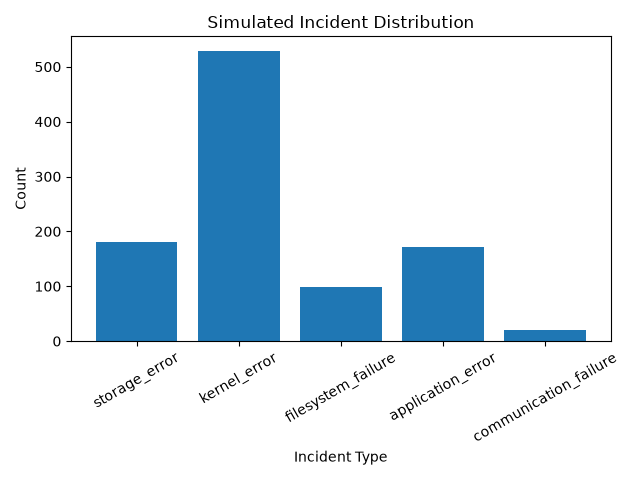
\includegraphics[width=\columnwidth]{figures/incident_distribution.png}
\caption{Incident distribution generated by the simulator for the 1,000-incident run.}
\label{fig:incident_distribution}
\end{figure}

\subsection{Outcome Model}
The simulator distinguishes three outcomes. RESOLVED indicates successful
remediation, RECURRED represents an action that appears to work but does not
resolve the underlying cause, and HARMFUL represents a remediation that makes
the simulated incident worse.

The fixed action-conditioned probabilities are:

\begin{table}[htbp]
\centering
\caption{Simulator Outcome Probabilities}
\label{tab:outcomes}
\begin{tabular}{lccc}
\toprule
Action & Resolved & Recurred & Harmful\\
\midrule
Restart service & 0.80 & 0.15 & 0.05\\
Requeue job & 0.45 & 0.35 & 0.20\\
Reset driver & 0.60 & 0.25 & 0.15\\
Drain node & 0.50 & 0.25 & 0.25\\
Reclaim disk & 0.40 & 0.30 & 0.30\\
\bottomrule
\end{tabular}
\end{table}

These probabilities are fixed simulator assumptions. They are not learned from
BGL and are not tuned during the benchmark to make EarnedAutonomy win.

\section{Implementation and Verification}
The core implementation is intentionally small. The gate is implemented in
\texttt{src/gate.py}, the Beta evidence model in \texttt{src/evidence.py}, and
incident and outcome simulation in \texttt{src/simulator.py}. Baseline policies
are in \texttt{src/baselines.py}; \texttt{benchmark.py} executes the controlled
comparison; and \texttt{threshold\_sweep.py} performs sensitivity analysis.

The final test suite contains 13 tests. It covers the no-history AUTO safety
condition, the high-blast-radius condition, PROPOSE and AUTO behavior, baseline
policy behavior, metric edge cases, benchmark determinism, unsafe-execution
counting, and the presence of the required audit fields in decision records.
The final run reported 13 passing tests.

The gate was also run against 1,000 incidents with no prior evidence. In that
state the lower evidence bound is insufficient for automatic execution, so the
initial gate verification produces zero AUTO decisions and keeps the decisions
under human control.

\section{Evidence Accumulation Experiment}
The learning experiment evaluates two known action contexts using 100 simulated
incidents per action and seed 42. The first context is restart service for a
kernel error on a compute node. The second is drain node for a communication
failure on a compute node.

The restart-service action begins without history and therefore starts at
ESCALATE. As outcomes are observed, successful observations increase the Beta
posterior and can move the decision through PROPOSE to AUTO. In the current
run, the first AUTO decision occurs at incident 16. Across the 100 simulated
incidents the decision counts are 3 ESCALATE, 50 PROPOSE, and 47 AUTO.

The drain-node action has a configured blast radius of 0.7, above the 0.60
risk ceiling. It therefore remains excluded from AUTO even when evidence is
accumulated. Its 100 decisions are all ESCALATE.

Figure~\ref{fig:auto_progression} plots the running proportion of AUTO
decisions. The plotted value is cumulative: it represents the fraction of
observed decisions classified as AUTO up to each incident.

\begin{figure}[htbp]
\centering
\includegraphics[width=\columnwidth]{figures/auto_decision_progression.png}
\caption{Running proportion of AUTO decisions during evidence accumulation. Restart service earns AUTO while drain node remains excluded by the risk ceiling.}
\label{fig:auto_progression}
\end{figure}

\begin{figure}[htbp]
\centering
\includegraphics[width=\columnwidth]{figures/week3_auto_proportion.png}
\caption{Week 3 AUTO proportion.}
\label{fig:week3_auto_proportion}
\end{figure}

This experiment satisfies the central earned-autonomy behavior required by the
design: one action progresses from ESCALATE to AUTO, while another never
becomes AUTO because of its risk profile.

\section{Experimental Methodology}
The benchmark compares three policies over the same deterministic incident
stream:

\begin{enumerate}
\item \textbf{Always Ask}: every candidate action receives human approval.
\item \textbf{Always Act}: every candidate action is executed automatically.
\item \textbf{EarnedAutonomy}: every candidate action passes through the trust gate.
\end{enumerate}

The four required metrics are defined as follows. Automatic resolution rate is
the proportion of all incidents whose action was both AUTO and resolved. Mean
time to recovery is the average simulated time from incident to final
resolution. Human interruptions count incidents requiring human involvement
before execution or during recovery. Unsafe automatic executions count AUTO
decisions followed by RECURRED or HARMFUL outcomes.

The benchmark models human approval as a fixed 120-second delay and human
recovery as a fixed 300-second delay. Action execution times are configured
per remediation type. These values are explicit simulation assumptions and
are held fixed during threshold sweeps.

The incident-to-action mapping is a lookup table. This is an explicit benchmark
assumption because BGL provides log observations rather than remediation
labels. The benchmark therefore tests the gate under a controlled ground-truth
simulation rather than claiming production remediation accuracy.

\section{Benchmark Results}

\subsection{Seed 42}
Table~\ref{tab:seed42} gives the benchmark results for the default deterministic
seed of 42.

\begin{table}[htbp]
\centering
\caption{Benchmark Results for Seed 42}
\label{tab:seed42}
\begin{tabular}{lrrrr}
\toprule
Policy & Auto Res. & MTTR (s) & Human & Unsafe Auto\\
\midrule
Always Ask & 0.000 & 291.685 & 1000 & 0\\
Always Act & 0.528 & 171.685 & 472 & 472\\
EarnedAutonomy & 0.000 & 443.905 & 1000 & 2\\
\bottomrule
\end{tabular}
\end{table}

Always Act provides the highest automation and the lowest mean recovery time
in this run, but it also produces 472 unsafe automatic executions. EarnedAutonomy
allows only two autonomous executions, both unsafe in this particular seed.
This is a deliberately important negative result: the gate is conservative,
but its current threshold does not guarantee zero unsafe executions.

Always Ask produces no unsafe automatic executions because it never executes
an action autonomously, but it also produces no automatic resolutions and
requires human involvement for all 1,000 incidents.

\subsection{Seed 43}
A second deterministic run uses seed 43. The results are shown in
Table~\ref{tab:seed43}.

\begin{table}[htbp]
\centering
\caption{Benchmark Results for Seed 43}
\label{tab:seed43}
\begin{tabular}{lrrrr}
\toprule
Policy & Auto Res. & MTTR (s) & Human & Unsafe Auto\\
\midrule
Always Ask & 0.000 & 288.300 & 1000 & 0\\
Always Act & 0.538 & 168.300 & 462 & 462\\
EarnedAutonomy & 0.011 & 442.320 & 989 & 0\\
\bottomrule
\end{tabular}
\end{table}

For seed 43, EarnedAutonomy performs 11 autonomous executions, achieves an
automatic resolution rate of 0.011, and records zero unsafe automatic
executions. Always Act again reaches 100\% automation but produces 462 unsafe
automatic executions.

The second seed therefore does not reverse the qualitative conclusion. The gate
remains much less autonomous than Always Act, while producing dramatically
fewer unsafe automatic executions in absolute terms.

\section{Threshold Sensitivity}
The threshold sweep evaluates AUTO thresholds from 0.50 to 0.95 and PROPOSE
thresholds from 0.20 to 0.50. Configurations where PROPOSE is greater than or
equal to AUTO are excluded, leaving 69 valid threshold combinations.

At PROPOSE=0.35 for seed 42, the selected AUTO-threshold results are shown in
Table~\ref{tab:sweep42}.

\begin{table}[htbp]
\centering
\caption{Selected Seed-42 Threshold Sweep Results at PROPOSE = 0.35}
\label{tab:sweep42}
\begin{tabular}{ccc}
\toprule
AUTO & Automation & Unsafe Auto\\
\midrule
0.50 & 3.7\% & 9\\
0.55 & 2.5\% & 7\\
0.60 & 1.1\% & 4\\
0.65 & 0.2\% & 2\\
0.70 & 0.0\% & 0\\
0.75 & 0.0\% & 0\\
0.80 & 0.0\% & 0\\
0.85 & 0.0\% & 0\\
0.90 & 0.0\% & 0\\
0.95 & 0.0\% & 0\\
\bottomrule
\end{tabular}
\end{table}

The threshold sweep shows the expected safety--automation trade-off. More
permissive AUTO thresholds increase autonomous execution, but they also
increase unsafe automatic executions in the seed-42 simulation. At thresholds
of 0.70 and above, no autonomous execution occurs in this run.

\begin{figure}[htbp]
\centering
\includegraphics[width=\columnwidth]{figures/automation_vs_unsafe_execution_seed42.png}
\caption{Automation--safety trade-off across threshold configurations for seed 42. The x-axis is automation rate and the y-axis is unsafe automatic execution rate.}
\label{fig:threshold42}
\end{figure}

The same sweep was executed with seed 43. At PROPOSE=0.35, the AUTO thresholds
0.50, 0.55, 0.60, 0.65, and 0.70 produce automation rates of 3.9\%, 2.8\%,
2.0\%, 1.1\%, and 0.7\%, respectively. The corresponding unsafe automatic
execution counts are 5, 3, 2, 0, and 0. This second sweep preserves the same
qualitative relationship between permissiveness and safety.

\begin{figure}[htbp]
\centering
\includegraphics[width=\columnwidth]{figures/automation_vs_unsafe_execution_seed43.png}
\caption{Automation--safety trade-off across threshold configurations for seed 43.}
\label{fig:threshold43}
\end{figure}

\section{Conditions Where EarnedAutonomy Does Not Dominate}
The experiments identify multiple conditions where EarnedAutonomy performs no
better than a baseline.

First, when the objective is minimum mean time to recovery and unsafe
automation is ignored, Always Act is better. For seed 42, Always Act reaches
171.685 seconds compared with 443.905 seconds for EarnedAutonomy. For seed 43,
the values are 168.300 and 442.320 seconds, respectively.

Second, when the objective is maximum automatic resolution rate, Always Act is
also better. Its automatic resolution rates are 0.528 and 0.538 for seeds 42
and 43, while EarnedAutonomy produces 0.000 and 0.011.

Third, at the default threshold in seed 42, EarnedAutonomy's two autonomous
executions are both unsafe. This shows that the gate's conservative automation
rate is not by itself sufficient to guarantee safe autonomy.

These limitations are useful results rather than failures to hide. The project
is designed to expose the trade-off between autonomy and safety, not to force
the proposed gate to outperform every baseline on every metric.

\section{Limitations and Threats to Validity}
The simulator is not a production infrastructure environment. Its action
outcome probabilities, action execution times, human delays, reversibility
values, and blast-radius values are modeling assumptions. They should not be
interpreted as production measurements.

The BGL dataset informs incident-frequency shape but does not provide
remediation ground truth. The benchmark therefore relies on a deterministic
incident-to-action lookup table. This provides controlled ground truth for
unsafe-execution measurement but limits external validity.

The evidence model treats resolved outcomes as successes and both recurrent
and harmful outcomes as failures. This is deliberately simple. Real systems
could distinguish partial recovery, repeated failure severity, or action-specific
costs, but adding those factors would exceed the project's defined scope.

The learning experiment allows supervised handling after ESCALATE or PROPOSE
to produce an outcome that contributes evidence. This models the practical
idea that human-approved remediation can still generate experience for future
autonomous decisions; it is not an assertion that the gate executed those
actions autonomously.

The current results use two deterministic seeds. They establish reproducible
behavior and a consistent qualitative trade-off, but they do not constitute a
statistical estimate of production performance.

\section{Safety Properties and Design Trade-offs}
The gate has two explicit safety properties that are tested directly. First,
an action with no observed history cannot receive AUTO. The initial Beta prior
therefore does not grant automatic permission by itself. Second, an action
whose normalized blast radius reaches the configured risk ceiling cannot
receive AUTO, even after successful observations. The tests exercise both
properties independently.

\subsection{No-History Constraint}
The no-history constraint addresses the uncertainty represented by the Beta
prior. With a Beta(1,1) prior, the posterior mean is 0.5, but that value does
not represent observed remediation performance. Using the lower fifth
percentile and additionally requiring observed history prevents the system from
interpreting the prior as empirical evidence. This makes the initial behavior
conservative and forces an action to accumulate observations before it can
cross the AUTO boundary.

\subsection{Blast-Radius Constraint}
The risk ceiling is an independent control from evidence. Drain-node has a
configured blast radius of 0.7 while the risk ceiling is 0.60. Consequently,
even a sequence of successful drain-node outcomes cannot satisfy the AUTO
condition. This separation is important because evidence answers whether an
action has worked before, whereas blast radius describes how costly an incorrect
action could be.

\subsection{Context-Specific Evidence}
Evidence is indexed by both action type and machine class. The design uses
three classes rather than individual machine identifiers so that the evidence
pool remains large enough to learn while retaining operational context. For
example, evidence for restart service on compute nodes is not automatically
used for restart service on storage nodes. This is a deliberate compromise
between over-generalization and excessively sparse evidence.

\subsection{Why the Gate Can Be Worse Than a Baseline}
The conservative design necessarily creates situations where EarnedAutonomy is
slower than Always Act. A PROPOSE or ESCALATE decision adds human delay even
when the underlying action would have succeeded. The current benchmark makes
this cost explicit through fixed human approval and recovery delays. This is
not an implementation defect hidden by the evaluation; it is the operational
price of reducing autonomous exposure.

The converse is also visible in the benchmark. Always Act has no mechanism to
use accumulated evidence, action reversibility, or blast radius to restrict
execution. It therefore achieves maximum automation but exposes every incident
to autonomous action. The comparison makes the project's intended design
trade-off measurable rather than assuming that either extreme is universally
correct.

\section{Detailed Benchmark Interpretation}
The four primary metrics are intentionally complementary. Automation rate measures
how often the gate permits autonomous execution, whereas automatic resolution
rate asks whether those autonomous executions actually resolve incidents.
Mean time to recovery captures the time cost of both automation and human
intervention. Human interruptions measures the operational burden placed on
people. Unsafe automatic executions directly measure the failure mode that the
trust gate is intended to control.

Table~\ref{tab:additional_metrics} reports the additional rates emitted by the
benchmark. These values are not used as replacements for the four required
metrics; they provide context for interpreting the primary results.

\begin{table}[htbp]
\centering
\caption{Additional Benchmark Metrics}
\label{tab:additional_metrics}
\begin{tabular}{lccc}
\toprule
Metric & Always Ask & Always Act & EarnedAutonomy\\
\midrule
\multicolumn{4}{c}{Seed 42}\\
\midrule
Automation rate & 0.000 & 1.000 & 0.002\\
Unsafe auto rate & 0.000 & 0.472 & 1.000\\
Remediation success & 0.528 & 0.528 & 0.528\\
\midrule
\multicolumn{4}{c}{Seed 43}\\
\midrule
Automation rate & 0.000 & 1.000 & 0.011\\
Unsafe auto rate & 0.000 & 0.462 & 0.000\\
Remediation success & 0.538 & 0.538 & 0.538\\
\bottomrule
\end{tabular}
\end{table}

The remediation success rate is equal across policies for a given seed because
the same simulated incident stream and action-conditioned outcome model are
used for the comparison. The policy changes the level of human involvement and
whether an outcome is classified as an unsafe autonomous execution; it does
not change the underlying simulator probabilities.

The seed-42 unsafe automatic execution rate for EarnedAutonomy is 1.000 even
though its automation rate is only 0.002. This distinction is important. A
small number of autonomous executions does not automatically imply that those
executions are safe. Conversely, seed 43 demonstrates that the same gate can
produce autonomous executions without an unsafe execution under a different
deterministic incident sequence.

\subsection{Decision Record Schema}
The benchmark stores structured records rather than only aggregate counts.
Table~\ref{tab:log_schema} summarizes the fields written for each simulated
decision.

\begin{table}[htbp]
\centering
\caption{Decision Record Fields}
\label{tab:log_schema}
\begin{tabular}{p{0.36\columnwidth}p{0.53\columnwidth}}
\toprule
Field & Purpose\\
\midrule
Timestamp & Time associated with the simulated incident\\
Incident ID/type & Identifies the incident and its category\\
Candidate action & Remediation selected by the lookup classifier\\
Machine class & Context used for evidence isolation\\
Reversibility & Action reversibility at decision time\\
Blast radius & Normalized action impact at decision time\\
Evidence lower bound & Conservative Beta-posterior evidence value\\
Trust and risk & Values used by the gate rule\\
Decision & AUTO, PROPOSE, or ESCALATE\\
Outcome/resolution & Observed result and resolution state\\
Recovery time & Simulated time from incident to final resolution\\
\bottomrule
\end{tabular}
\end{table}

This schema allows a reviewer to trace an aggregate benchmark metric back to
the underlying simulated decisions. It also makes the distinction between the
policy decision and the eventual outcome explicit.

\section{Reproducibility}
The repository uses Python 3.10 or newer and requires pytest, matplotlib,
SciPy, and PyYAML. The core gate remains a small set of Python
modules without a heavy framework.

The benchmark is run with:

\begin{verbatim}
python benchmark.py
\end{verbatim}

A second seed is run with:

\begin{verbatim}
python benchmark.py --seed 43
\end{verbatim}

Threshold sensitivity is reproduced with:

\begin{verbatim}
python threshold_sweep.py --seed 42
python threshold_sweep.py --seed 43
\end{verbatim}

The evidence accumulation experiment is reproduced with:

\begin{verbatim}
python run_learning_experiment.py
\end{verbatim}

The test suite is run with:

\begin{verbatim}
python -m pytest -q
\end{verbatim}

The final verification reported 13 passing tests. Benchmark outputs are stored
as seed-specific JSON files, and the default seed-42 command also writes the
repository-level benchmark result and summary files. The four paper figures
are stored in \texttt{figures/}.

\section{Conclusion and Future Work}
EarnedAutonomy implements a small trust gate that makes autonomous remediation
conditional on reversibility, blast radius, and accumulated context-specific
evidence. The Beta posterior lower bound provides a conservative evidence score,
while the explicit risk ceiling prevents high-blast-radius actions from
becoming AUTO solely because of historical success.

The controlled learning experiment demonstrates earned autonomy: restart
service progresses from ESCALATE through PROPOSE to AUTO, while drain node
remains excluded from AUTO. The benchmark demonstrates the central trade-off.
Always Act is faster and more autonomous but generates hundreds of unsafe
automatic executions. EarnedAutonomy is substantially less autonomous and
slower, but its unsafe automatic execution count is much lower in absolute
terms across the two evaluated seeds.

The threshold sweep further shows that autonomy cannot be increased for free.
Lower AUTO thresholds increase autonomous execution and, in the seed-42 run,
increase unsafe automatic executions. The results therefore support a
safety-first interpretation of earned autonomy rather than an automation-first
one.

Future work within a production setting would require calibrated risk values,
production remediation outcomes, and broader evaluation across infrastructure
contexts. Those extensions are outside the present simulator-based scope. The
current artifact instead provides a small, reproducible, and inspectable gate
and benchmark that makes its assumptions and limitations explicit.

\begin{thebibliography}{00}

\bibitem{kephart}
J. O. Kephart and D. M. Chess,
``The vision of autonomic computing,''
\textit{Computer}, vol. 36, no. 1, pp. 41--50, 2003,
doi: 10.1109/MC.2003.1160055.

\bibitem{huebscher}
M. C. Huebscher and J. A. McCann,
``A survey of autonomic computing---degrees, models, and applications,''
\textit{ACM Computing Surveys}, vol. 40, no. 3, 2008,
doi: 10.1145/1380584.1380585.

\bibitem{ghosh}
D. Ghosh, R. Sharman, H. Raghav Rao, and S. Upadhyaya,
``Self-healing systems---survey and synthesis,''
\textit{Decision Support Systems}, vol. 42, no. 4, pp. 2164--2185, 2007,
doi: 10.1016/j.dss.2006.06.011.

\bibitem{macias}
F. D. Macías-Escrivá, R. Haber, R. del Toro, and V. Hernández,
``Self-adaptive systems: A survey of current approaches, research challenges
and applications,''
\textit{Expert Systems with Applications}, vol. 40, no. 18,
pp. 7267--7279, 2013, doi: 10.1016/j.eswa.2013.07.033.

\bibitem{krupitzer}
C. Krupitzer, F. M. Roth, S. VanSyckel, G. Schiele, and C. Becker,
``A survey on engineering approaches for self-adaptive systems,''
\textit{Pervasive and Mobile Computing}, vol. 17, pp. 184--206, 2015,
doi: 10.1016/j.pmcj.2014.09.009.

\bibitem{wong}
T. Wong, M. Wagner, and C. Treude,
``Self-adaptive systems: A systematic literature review across categories and
domains,''
\textit{Information and Software Technology}, vol. 148, 106934, 2022,
doi: 10.1016/j.infsof.2022.106934.

\bibitem{oliner}
A. J. Oliner and J. Stearley,
``What supercomputers say: A study of five system logs,''
in \textit{Proc. IEEE/IFIP International Conference on Dependable Systems and
Networks}, pp. 575--584, 2007, doi: 10.1109/DSN.2007.103.

\bibitem{loghub}
J. Zhu, S. He, P. He, J. Liu, and M. R. Lyu,
``Loghub: A large collection of system log datasets for AI-driven log analytics,''
in \textit{Proc. IEEE International Symposium on Software Reliability Engineering},
pp. 355--366, 2023, doi: 10.1109/ISSRE59848.2023.00071.

\bibitem{drain}
P. He, J. Zhu, Z. Zheng, and M. R. Lyu,
``Drain: An Online Log Parsing Approach with Fixed Depth Tree,''
in \textit{Proc. IEEE International Conference on Web Services},
pp. 33--40, 2017, doi: 10.1109/ICWS.2017.13.

\bibitem{virtanen}
P. Virtanen et al.,
``SciPy 1.0: Fundamental algorithms for scientific computing in Python,''
\textit{Nature Methods}, vol. 17, pp. 261--272, 2020,
doi: 10.1038/s41592-019-0686-2.

\bibitem{edge_review}
L. Bonilla Viana, J. Diaz-de-Arcaya, J. Aguirre Usandizaga, and A. Almeida,
``AI-driven self-healing across the edge--cloud continuum: A systematic
literature review,''
\textit{Information and Software Technology}, vol. 198, 108232, 2026,
doi: 10.1016/j.infsof.2026.108232.

\end{thebibliography}

\end{document}